\documentclass[a4paper]{scrartcl}
\usepackage[cm]{fullpage}
\usepackage{amsmath, amssymb, esint}
\usepackage[backend = biber, style = numeric-comp]{biblatex}

\usepackage{cancel}
\usepackage{fixltx2e}
\usepackage{wrapfig, subcaption, caption}

\usepackage{sectsty}
\sectionfont{\large\selectfont}
\subsectionfont{\normalsize\selectfont}

\usepackage{tikz, pgfplots}
\pgfplotsset{compat = 1.9}

\usepackage{siunitx}

\begin{filecontents}{\jobname.bib}
@article{Swalen1962,
    doi = {10.1063/1.1701290},
    url = {http://dx.doi.org/10.1063/1.1701290},
    year  = {1962},
    publisher = {{AIP} Publishing},
    volume = {36},
    number = {7},
    pages = {1914},
    author = {J. D. Swalen and James A. Ibers},
    title = {Potential Function for the Inversion of Ammonia},
    journal = {The Journal of Chemical Physics}
}
\end{filecontents}
\addbibresource{\jobname.bib}

\begin{document}

\title{PHYS2111: Assignment 2}
\author{ \\ \\ }
\date{2016-05-19}
\maketitle

\section{Consider a beam of particles incident on a step in potential. The step in potential is described by the function \(V(x) = V_0 \theta(x)\) where \(\theta\) is the Heaviside step function.}
\subsection{The particles have an energy \(E\), which is greater than \(V_0\). Starting with the solution to the TISE for a free particle, show that the solutions to the TISE for this situation are: where \(x < 0\), \(\psi_1(x) = A e^{i k_1 x} + B e^{-i k_1 x}\); where \(x > 0\), \(\psi_2(x) = C e^{i k_2 x} + D e^{-i k_2 x}\); where \(A\), \(B\), \(C\) and \(D\) are constants.}
Since the potential has a discontinuity at \(x = 0\), we can divide the potential into two parts: \(x < 0\) and \(x > 0\) and solve them independently.

Since both parts have potentials lower than the particles' energy, they are free particles on both sides of the potential and so their wavefunctions are identical to that of a free particle:
\[\psi(x) = C_1 e^{i k x} + C_2 e^{-i k x}\]

Using this equation and solving the TISE with our potential results in:
\[
    k =
    \begin{cases}
        \sqrt{\frac{2 m E}{\hbar^2}} & \text{if } x < 0 \\
        \sqrt{\frac{2 m (E - V_0)}{\hbar^2}} & \text{if } x > 0
    \end{cases}
\]

Labelling the \(x < 0\) wavefunction to be \(\psi_1\) and the \(x > 0\) to be \(\psi_2\), and renaming the constants to \(A\), \(B\), \(C\) and \(D\), we get the solutions as required:
\begin{align*}
    \psi_1(x) &= A e^{i k_1 x} + B e^{-i k_1 x} \\
    \psi_2(x) &= C e^{i k_2 x} + D e^{-i k_2 x}
\end{align*}
Where:
\begin{align*}
    k_1 &= \sqrt{\frac{2 m E}{\hbar^2}} \\
    k_2 &= \sqrt{\frac{2 m (E - V_0)}{\hbar^2}}
\end{align*}

\subsection{Now turn your equations from above into time varying equations, justifying the steps, and explain the meaning of all terms.}
Since the TISE was derived by assuming \(V\) to be time-independent and setting \(\Psi(x, t) = \psi(x) \tau(t)\), where \(\Psi\) is the full (time varying) wavefunction, \(\psi\) the time-independent component and \(\tau\) the time-dependent component, we can always recover the time varying wavefunction by multiplying our time-independent solution by \(\tau\).

\(\tau\) can be trivially shown to always equal \(e^{\frac{-i E t}{\hbar}}\) for the non-relativistic Schrodinger equation, where \(E\) is the total energy of the particle.

Therefore, the time varying equations for our system are:
\begin{align*}
    \Psi_1(x) &= \left(A e^{i k_1 x} + B e^{-i k_1 x}\right) e^{\frac{-i E t}{\hbar}} \\
    \Psi_2(x) &= \left(C e^{i k_2 x} + D e^{-i k_2 x}\right) e^{\frac{-i E t}{\hbar}}
\end{align*}

\subsection{Find values for \(A\), \(B\), \(C\) and \(D\).}
Since the particles are incident from the left, there are no particles arriving from the right, therefore \(D\) must equal 0.

Since a wavefunction with finite potentials has to be in \(C^1\), we can also examine the boundary conditions at \(x = 0\):
\begin{align*}
    &\begin{cases}
        \psi_1(0) = \psi_2(0) \\
        \frac{\mathrm{d}}{\mathrm{d}x} \psi_1(0) = \frac{\mathrm{d}}{\mathrm{d}x} \psi_2(0)
    \end{cases} \\
    \therefore &\begin{cases}
        A + B = C + D = C \\
        k_1 (A - B) = k_2 (C - D) = k_2 C
    \end{cases} \\
    \therefore &B = A \frac{k_1 - k_2}{k_1 + k_2} \\
    &C = A \frac{2 k_1}{k_1 + k_2}
\end{align*}

Where \(A\) remains as an arbitrary constant.

\subsection{Show that we can define \(R = \frac{|B|^2}{|A|^2} = \frac{(k_1 - k_2)^2}{(k_1 + k_2)^2}\) and \(T = \frac{k_2 |C|^2}{k_1 |A|^2} = \frac{4 k_1 k_2}{(k_1 + k_2)^2}\) and verify that \(T + R = 1\).}
\(R = \frac{|B|^2}{|A|^2}\) is clearly \(\frac{(k_1 - k_2)^2}{(k_1 + k_2)^2}\) from the previous question. For \(T\):
\begin{align*}
    T &= \frac{k_2 |C|^2}{k_1 |A|^2} = \frac{k_2}{\cancel{k_1}} \frac{4 k_1^{\cancel{2}}}{(k_1 + k_2)^2} \\
    &= \frac{4 k_1 k_2}{(k_1 + k_2)^2}
\end{align*}

Adding them together reveals:
\begin{align*}
    T + R &= \frac{(k_1 - k_2)^2 + 4 k_1 k_2}{(k_1 + k_2)^2} \\
    &= \frac{(k_1 + k_2)^2}{(k_1 + k_2)^2} \\
    &= 1
\end{align*}

\subsection{Now assume that the beam of particles has \(E < V_0\). Where \(x > 0\), the wave function is given by \(\psi(x) = C e^{i k_2 x} = C e^{-\alpha x}\) where \(\alpha = \sqrt{\frac{2 m (V_0 - E)}{\hbar^2}}\). Now assume each electron in the beam has energy \(E = 0.1 V_0\), and that the beam is incident on a potential step of \(V_0 = \SI{2}{\electronvolt}\). Graph the relative probability \(\psi^2\) of particles penetrating the step up to a distance of \(x = \SI{e-9}{\metre}\).}
With the electron mass \(m = \SI{9.109e-31}{\kilo\gram}\), we get \(\alpha = \SI{6.873e9}{\per\metre}\).

\begin{figure}[h]
    \centering
    \begin{tikzpicture}
        \begin{axis}[
            xlabel = \(x \times \SI{e-9}{\metre}\),
            ylabel = Relative Probability,
            width = 18cm,
            height = 10cm,
            samples = 100
        ]
            \def\alpha{6.873}
            \addplot[color = blue, domain = 0:1] {e^(-2 \alpha * x)};
        \end{axis}
    \end{tikzpicture}
\end{figure}

\section{The ammonia (NH\textsubscript{3}) molecule has a periodic \emph{inversion} transition that makes it highly useful as both an atomic clock, and as a way of measuring the temperature in interstellar molecular clouds.}
\subsection{Describe the two equilibrium configurations of NH\textsubscript{3} (use diagrams).}
\begin{wrapfigure}[2]{r}{5cm}
    \centering
    \vspace{-1cm}
    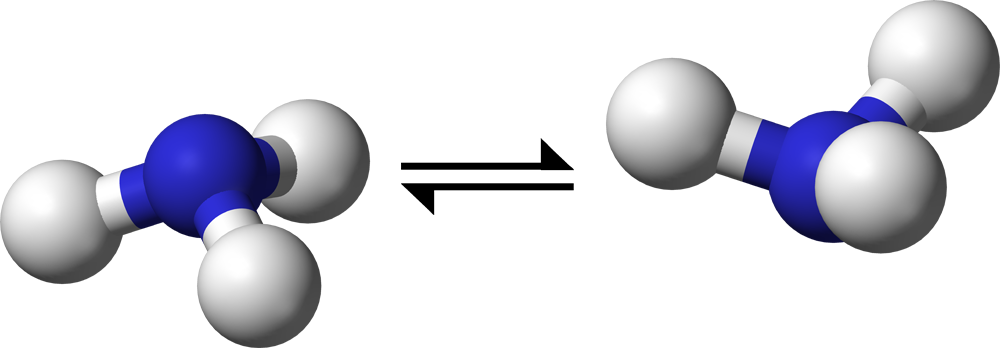
\includegraphics[width = 5cm]{ammonia-inversion.png}
\end{wrapfigure}
The two equilibrium configurations occur when either the nitrogen atom is above or below the plane of hydrogens.

\subsection{Draw a potential energy diagram of the NH\textsubscript{3} molecule as seen by the nitrogen atom along a line perpendicular to the symmetry plane. Clearly mark the position of the two equilibrium points (\(-a\), \(+a\)) on the spatial dimension of your diagram, which should be perpendicular to the symmetry plane. Show this spatial axis on a diagram of the NH\textsubscript{3} molecules, clearly marking the symmetry plane.}
\begin{figure}[h]
    \centering
    \begin{subfigure}{0.5 \textwidth}
        \begin{tikzpicture}
            \begin{axis}[
                xlabel = \(z\) (Arb.),
                ylabel = \(V\) (Arb.),
                xtick = {-1, 1},
                xticklabels = {\(-a\), \(a\)},
                ymajorticks = false,
                samples = 100
            ]
                \addplot[color = blue, domain = -1.6:1.6] {(x^2 - 1)^2};
            \end{axis}
        \end{tikzpicture}
    \end{subfigure}
    \begin{subfigure}{0.2 \textwidth}
        \centering
        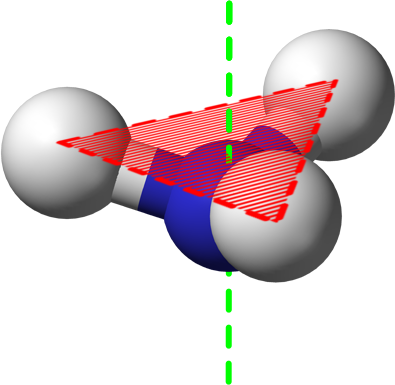
\includegraphics[width = \textwidth]{ammonia-inversion-axis.png}
        \caption*{Red: Symmetry Plane\\ Green: \(z\)-axis}
    \end{subfigure}
\end{figure}

\subsection{Explain qualitatively why the inversion transition involves quantum tunnelling.}
Assuming the ammonia molecule is at a sufficiently low temperature that the nitrogen atom has less energy than the inversion barrier, and there are no external inputs of energy, it classically cannot invert and is localised within one or the other equilibrium state.

However, experimentally, it can be found that the nitrogen atom oscillates between both states when energy smaller than the potential barrier is applied (e.g., with a photon), which can only mean it is the effect of quantum tunnelling.

\subsection{Estimate the tunnelling probability and rate for the N atom.}
\emph{Note: This question appears to have been taken from \emph{Modern Physics 3rd. Edition} by Serway, Moses and Moyer, but using their specified values and working resulted in more than an order of magnitude error in the oscillation frequency, so I have used a different method.}

Swalen \cite{Swalen1962} provides an empirical potential function for ammonia inversion:
\[V(\theta) = 24245 \theta^2 + 12438 \theta^4 + 12344 e^{-4.369 \theta^2} \si{\per\centi\metre}\]
where \(\theta\) is the angle between the hydrogen plane and the N-H bonds. Note that the minimum potential is greater than 0.

They also provided some empirically determined values that we will be using as well:
\begin{align*}
    r_c &= \SI{1.0116}{\angstrom} \\
    \mu &= \SI{2.561}{\amu} = \SI{4.251e-24}{\gram}
\end{align*}
where \(r_c\) is the N-H bond length in the equilibrium state, and \(\mu\) the reduced mass of the nitrogen atom together with the hydrogen plane.

From their results, they determined that the N-H bond length mostly does not change during the transition, so we can represent the potential in terms of the linear Cartesian \(z\)-axis:
\[V(z) = V\left(\theta = \sin^{-1}\frac{z}{r_c}\right)\]

Solving the TISE numerically with this potential for the two lowest bound states results in \(E_0 = \SI{10879.90}{\per\centi\metre}\) and \(E_1 = \SI{10881.01}{\per\centi\metre}\). If we take the average of these two as \(E = \SI{10880.46}{\per\centi\metre}\), we can use the WKB approximation to estimate the tunnelling probability:
\[T \approx \exp\left(-2 \int_{z_1}^{z_2} \sqrt{\frac{2 \mu}{\hbar^2} (V(z) - E)} \:\mathrm{d}z\right)\]

\(z_1\) and \(z_2\) are the classical turning points of the particle (i.e., \(V(z) = E\)) and are at \(-z_1 = z_2 = \SI{0.2604}{\angstrom}\) for our \(E\). Evaluating the integral numerically then gives:
\[T \approx e^{-11.661} \approx \SI{8.6235e-6}{}\]

As for the tunnelling rate, semi-classically, this is proportional to the width of the line split caused by the tunnelling (i.e., the difference between the first two bound state energies):
\[\nu = \frac{E_1 - E_0}{h} \approx \SI{33}{\giga\hertz}\]

Unfortunately, this is different to the expected \SI{24}{\giga\hertz}, and as mentioned in Swalen's paper, is because the potential function does not fit very well at the low energy bound states.

\printbibliography

\end{document}
